\chapter{Implementation}
This chapter explains the different phases of the \lang{} compiler, and how they were implemented for the \lang{} compiler. The \lang{} compiler has several distinct phases, as seen on \ref{fig:compphase}. 


\begin{figure}[H]
    \centering
    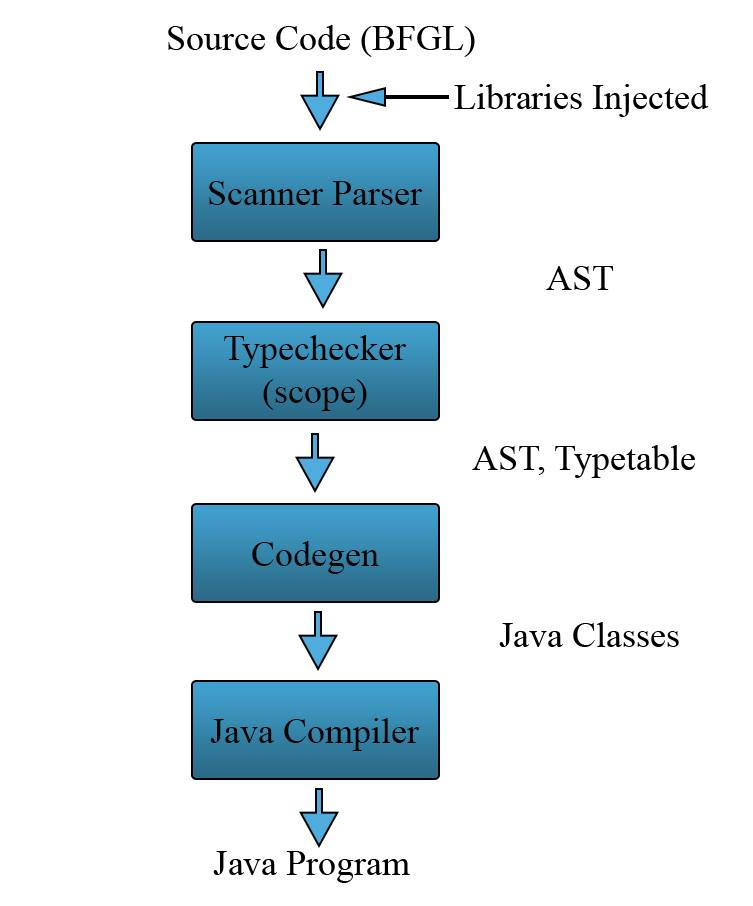
\includegraphics[scale=0.5]{resources/Images/compiler-phase.jpeg}
    \caption{A generalized figure of the phases of the \lang{} compiler.}
    \label{fig:compphase}
\end{figure}

These phases are:

\begin{itemize}
    \item Library injection
    \item Scanner and Parser
    \item Type checker
    \item Code generator
    \item Java Compiler
\end{itemize}

The \lang{} compiler, as a whole, takes a file with code written in \lang{} as input and outputs an executable Java program.

The first thing that happens when a user wants to compile a \lang{} file in the \lang{} compiler, is that the \lang{} libraries are injected into the user's file. This is done to include the libraries in the AST, so that they are present when the type checker is run.

After the libraries are added to the source file, the file is run through the scanner and parser, which is generated by SableCC. This phase returns an AST of the program, which is used throughout the rest of the compiler.

The next phase, the type checker, performs a tree walk of the AST. During the walk, the type checker adds each node to a hash table with a reference to the node and the type of the node, adds all variables, methods and classes to a symbol table, validates the types of a node's child nodes and checks if the different variables, methods and classes are within the scope. When the type checking phase is complete, it is known whether or not the \lang{} program is semantically correct. The type table is also returned for use in the code generation phase of the compiler.

When the source program is confirmed to be a valid program in \lang{}, the code generation phase is initiated. In this phase, a new tree walk is done over the AST and code is generated for each node. When this phase is completed, a number of java files have been generated, which is afterwards run trough the final phase of the compiler, namely the Java Compiler.

The following sections gives a more in-depth explanation of the different phases of the \lang{} compiler, but before that, the Depth First adapter, used for the different tree walks, is explained.

\section{SableCC's Depth first adapter}
SableCC provides a depth first adapter class, which is intended to be used in later phases of the compiler to traverse the AST for analysis and code-generation purposes. When implementing the analysis and codegen phases, the depth-first adapter class can simply be extended, which, in the end, saves development time and reduces the amount of errors that could be introduced when implementing the compiler. The adapter implements two functions for each Node type in the AST. These are an \textit{in} and \textit{out} function. The \textit{in} function is called each time the tree walker enters, i.e the first time it visits a node, and the \textit{out} function is called when the tree walker has visited the whole sub-tree rooted in that node, i.e when it exits a node. An example template of how these \textit{in} and \textit{out} functions could look for a "Prog" node, which is always the first node to be created in the AST, is shown below:
\begin{figure}[H]
    \centering
    
    \begin{lstlisting}[style=gglang]
    public void inAProg(AProg node){
        
        //Some code to be executed on node entry here
    
    }
    public void outAProg(Aprog node){
    
        //Some code to be executed on node exit here
        
    }
    
    \end{lstlisting}
    \caption{Example for how the in and out methods are used in the \lang{} compiler\label{fig:inout}}
\end{figure}
There is of course a lot of other nodes, which can be found in the AST grammar in appendix \ref{AST}.
The different kinds of actions, that are needed in the analysis and code generation phases, are hereafter implemented as extensions of the DepthFirstAdapter class. This approach is used through the rest of the compiler. 

\section{Scanner and Parser phase}

The scanner (also known as the lexer) and parser used for \lang{} has been generated using SableCC, with a modified version of the grammar shown in Section \ref{sec:OurSyntax}. The actual code used with SableCC can be found in \ref{FGramma}. By running code in \lang{} through the parser, an Abstract Syntax Tree (AST) is generated, which will then be used in the semantic analysis phase, and in the code-generation phase.
The grammar definition is split into two parts. The first part defines the syntax of \lang{} and aids the creation of a CST structure, and the second part defines an AST structure for input generated by the first phase of the compiler. The CST is used internally by the code generated by SableCC, and is never touched in the implementation of \lang{}. The AST, however, is the result the syntax analysis phase produces, and it is what is used further on in the following phases. 
The grammar for the AST and the CST are very similar. The main difference is that the AST grammar can be ambigious, whereas the CST grammar must be unambigous. Both grammars can be found in the appendix, AST grammar at appendix \ref{AST}, and the CST at the top of appendix \ref{FGramma}. They are both written in the style required by SableCC, although still close to the original grammar.
\subsection{Implementation of Syntax in \lang{}}
The implementation of \lang{}'s syntax is handled entirely by SableCC, as it generates both the lexer and the parser. There is no custom code in this part of the compiler. It is all generated by SableCC. The only "custom" code is an object instance which contains the AST after being produced by the lexer/parser. The code used for calling the parser and lexer is implemented as follows:
\begin{figure}[H]
    \centering
    
    \begin{lstlisting}[style=gglang]
        PushbackReader pushbackReader = new PushbackReader(new FileReader(addLibrary(file)));
        Parser parser = new Parser(new Lexer(pushbackReader));
        Start tree = parser.parse();
    \end{lstlisting}
    \caption{The code for calling the parser and lexer.\label{fig:parslex}}
\end{figure}
"PushbackReader" is the lexer, and "Parser" is the parser. "tree" is the object instance containing the AST after the parser is done. 
\section{Type checker phase}
\label{sec:semanticAnal}
Besides generating a parser, SableCC also generates a \textit{tree walking} class, which can traverse the AST. This is done using a modified version of the visitor pattern, implemented by SableCC. 

To implement the type and scoping rules, defined formally in chapter \ref{chap:semantics}, a new class has been created, called \textit{TypeChecker}. This class inherits from a class generated by SableCC, called \textit{DepthFirstAdapter}, as described in the introduction to this chapter.  The \textit{in} and \textit{out} functions, that is described for all Nodes, will be used to implement the type and scoping rules. 

\subsection{Symbol table and scope}
The symbol table is implemented as a stack of \textit{hash tables}, indexed by an id string, i.e. the id of the variable or function in question, and value of a reference to the node where it is declared. Each time a new scope is opened, a new \textit{hash table} is pushed to the stack, and when a scope is closed, the hash table on top of the stack is removed. This makes sure that the current scope is always on top of the stack, and that only the nodes in scope are located in memory. 


\begin{figure}[H]
\centering
\begin{lstlisting}[]

    private void openScope(Node node){
        TableFiller tf = new TableFiller(node);

        node.apply(tf);

        symStack.push(tf.symStack.pop());
        typeTable.putAll(tf.typeTable);
        ErrorList.addAll(tf.ErrorList);
    }
    
\end{lstlisting}
\caption{Code example: \textit{openScope}}
\label{fig:openscope}
\end{figure}

When a new scope is opened, the function shown on figure \ref{fig:openscope} is called. This function initiates a new instance of the \textit{TableFiller} class, which also inherits from the \textit{DepthFirstAdapter}. When the TableFiller object is applied to a node, as seen on line 5 of figure \ref{fig:openscope}, it initiates a tree walk over the subtree with that node as the root. During this tree walk, it fills its own symbol table, by adding to it each time it encounters a declaration node. This symbol table is then popped, and the result is added to the actual symbol table stack, as seen on line 7.

This pass is done to make it possible to call a function or class that has not yet been declared in the code.

The TableFiller class implements \textit{out} functions for all the declaration nodes and \textit{in} functions for some of them.

To add a symbol to the symbol table, a function called addSymbol is called. This function is seen on figure \ref{fig:addsymbol}. The \textit{addSymbol} function takes a name and a node as parameters. These are the values that are added to the symbol table.

\begin{figure}[H]
\centering
\begin{lstlisting}[]

    private void addSymbol(String name, Node node){
        if (!symStack.peek().containsKey(name)) {
            symStack.peek().put(name, node);
        }
        else
            ErrorList.add("ERROR: " + name + " is already defined in this scope " + symStack.peek().size());
    }
    
\end{lstlisting}
\caption{Code example: \textit{addSymbol}}
\label{fig:addsymbol}
\end{figure}

Before adding the symbol to the symbol table, the function first makes a check to see if the symbol is already in the current scope (the symbol can be in an outer scope, since \lang{} has symbol shadowing). If the symbol is not found in the current scope, it is added, as seen on line 4 of figure \ref{fig:addsymbol}. If it is already in the current scope, an error message is added to an ArrayList called \textit{ErrorList}, which is a list of all the errors found. This will be used later on for displaying error messages.

To implement the dot operator, i.e '\textit{object\textbf{.}attribute}', the scope analyser must traverse the declaration sub tree for the class to check that it implements the attribute in question. This is done by applying the \textit{TableFiller} on the root of the class declaration sub tree. If a there are more than one level or more than one 'dot' in a call made with the dot operator, a new scope is opened for each class in the call with the current scope being the right most class in the call.



\subsection{Type Checker}
To implement the type rules, a new \textit{hash table} is used. This table is indexed by a node reference and its value is a string containing the type of that node. The value is a string and not a enum type, since in \lang{} the user can implement their own types. 

When talking about type checking, the nodes of the AST can be divided into four different categories, namely;

\begin{itemize}
    \item Nodes with no type.\\
    \textit{i.e main- and event-nodes}
    
    \item Nodes with a type. \\
    \textit{i.e value- and type-nodes}
    
    \item Nodes with a type, that is dependent of its child nodes.\\
    \textit{i.e function declaration- and expression-nodes}
    
    \item Nodes with no type, but with child nodes of a certain type.\\
    \textit{i.e if- and loop-nodes}
\end{itemize}

These different nodes are handled in different ways in the implementation of the type checker.

The first category of nodes are not handled in the type checking phase, since the nodes themselves always will be type-correct, and the type correctness of the child nodes will be validated on their respective nodes.

The second categories of nodes must be added to the type table. This is done by calling the function \textit{addType}, as seen on figure \ref{fig:addtype}. The call is made in the \textit{out} function of a node. The \textit{addType} function simply adds the node to the \textit{typeTable}. It is necessary to call \textit{trim()}, which removes white space at the start and end of the string.


\begin{figure}[H]
\centering
\begin{lstlisting}[]
    private void addType(Node node, String type){
        typeTable.put(node, type.trim());
    }
    
\end{lstlisting}
\caption{Code example: \textit{addType}}
\label{fig:addtype}
\end{figure}

An example of an \textit{out} function, as explained in \ref{sec:semanticAnal}, for a node in the second category can be seen on figure \ref{fig:outAFuncCall}.

\begin{figure}[H]
\centering
\begin{lstlisting}[]
    public void outAFuncCall(AFuncCall node){
        addType(node, getType(node.getId().getText()));
    }
    
\end{lstlisting}
\caption{Code example: \textit{outAFuncCall}}
\label{fig:outAFuncCall}
\end{figure}

Figure \ref{fig:outAFuncCall} shows how a node is added to the type table. In this example, the type is found by calling \textit{getType}, which searches the type-table. Some nodes, such as the different \textit{type} nodes, simply adds the string of their type.

The third category of nodes are the nodes whose type is dependent on the type of their child nodes. These include, but are not limited to, expression nodes.

Firstly, the child nodes' type is checked to evaluate if they meet the specification made in \ref{sec:TypeRules}. An example can be seen in the \textit{out} function of the \textit{plus-expression} node, as seen on figure \ref{fig:outAPlusExpr}.


\begin{figure}[H]
\centering
\begin{lstlisting}[]
    public void outAPlusExpr(APlusExpr node){
        if(typeTable.get(node.getLeft()).equals(TEXT) || typeTable.get(node.getRight()).equals(TEXT)){
            addType(node, TEXT);
        }
        else if(typeTable.get(node.getLeft()).equals(NUM)){
            if(typeTable.get(node.getRight()).equals(NUM)){
                addType(node, NUM);
            }
            else{
                ErrorList.add("ERROR line " + lineAndPos.getLine(node) + " pos " + lineAndPos.getPos(node) + " : " + node.getRight().toString() + ", is not of type " + NUM + ".");
                addType(node, ERRORTYPE);
            }
        }
        else{
            ErrorList.add("ERROR line " + lineAndPos.getLine(node) + " pos " + lineAndPos.getPos(node) + " : " + node.getLeft().toString() + ", is not of type " + NUM + ".");
            addType(node, ERRORTYPE);
        }
    }
    
\end{lstlisting}
\caption{Code example: \textit{outAPlusExpr}}
\label{fig:outAPlusExpr}
\end{figure}

In this example, if either of the child nodes are of type \textit{text}, the type of the whole expression is \textit{text}. The same goes for \textit{num}. If both these cases are false, an error is added to the ErrorList and the node gets the type \textit{ERRORTYPE}. This is done to allow the compiler to continue and collect all the errors, instead of stopping at the first type error encountered.

The fourth and last category of nodes are the nodes that are dependent on the type of one or more of their child nodes, but do not have a type themselves.

\begin{figure}[H]
\centering
\begin{lstlisting}[]
    public void outAForupStmt(AForupStmt node){
        closeScope();

        if(!typeTable.get(node.getExpr()).equals(NUM)){
            ErrorList.add("ERROR line " + lineAndPos.getLine(node.getExpr()) + " pos " + lineAndPos.getPos(node.getExpr()) + " : " + node.getExpr().toString() + ", is not of type " + NUM + ".");
        }

        if(!getType(node.getId().getText()).equals(NUM)){
            ErrorList.add("ERROR line " + lineAndPos.getLine(node.getId()) + " pos " + lineAndPos.getPos(node.getId()) + " : " + node.getId().toString() + ", is not of type " + NUM + ".");
        }
    }
    
\end{lstlisting}
\caption{Code example: \textit{outAForupStmt}}
\label{fig:outAForupStmt}
\end{figure}

An example of such a node is the \textit{ForupStmt} node. The \textit{out} function for this can be seen on figure \ref{fig:outAForupStmt}. This function only needs to control the types of the child nodes and thus not add anything to the type table.

Due to the fact that a function's type is not declared on the function declaration in \lang{}, the return type of the function must be found by examining the return node of the function declaration. To achieve this, the function declaration sub tree is traversed by applying the TypeChecker to the function declaration node. The type is then set to the type of the return node's expression child node. 

\subsubsection{Inheritance}
To obtain the inherited type of an object, it is necessary to add a new table, namely a super table. Each entry in the table contains two strings; one for the object's own type and one for the super type.

\subsubsection{Error handling}
If an error is encountered during compilation, one of two things can happen. If the error originates from the lexer/parser part of the compiler, for example a syntactical error, it is shown on the GUI, and compilation will be terminated. If the error, on the other hand, is from the semantic/contextual analysis phase, for example a semantic error, it is added to a List called errorlist, and the whole list is shown once the compilation is done or has reached a point where it cannot continue.

This concludes the section about the type-checker itself. The following chapter is about code-generation, and how it was implemented for the \lang{} compiler. 

\section{Code Generation phase}
The last phase of the compiler is the code-generation phase. In this phase, code is generated for the target language, which, in the case of \lang{}, is Java. The code generation is done using the AST produced by the previous compiler phases, and using the Sable-CC tree-walking method similarly as done in the previous phases. The code that calls the JavaCodeGenerator class to begin code generation for java is implemented as seen on figure \ref{fig:startcodegen}.

\begin{figure}[H]
    \centering
    
    \begin{lstlisting}[style=gglang]
            new JavaCodeGenerator(typeChecker.typeTable, typeChecker.superTable, tree);
            AntExecutor AEx = new AntExecutor();
            AEx.executeAntTask("CompileBFGL.xml", "jar");
    \end{lstlisting}
    \caption{The code for calling the class responsible for starting code generation.\label{fig:startcodegen}}
\end{figure}
The last two lines are not directly responsible for generating java code, but they execute the rest of the build process. This includes moving library-files to the right positions, calling the java compiler to compile the generated java code to .class files, and finally creating an executable .jar file with the compiled game contained inside.

\subsection{Code Generation for Java}
To accommodate the different needs of an object-oriented language, six different visitors were created based on the depth-first adapter from Sable-CC.
This uses the \textit{in} and \textit{out} functions, just like the semantic analysis did in the last section, as shown on \ref{fig:inout}.


\subsubsection{JavaCodeGenerator}
An instance of this class is created at the beginning of the codegen phase. The first thing it does is to add in some of the libraries contained in the Libraries folder, which is implemented as seen on figure \ref{fig:librarycodegen}.
\begin{figure}[H]
    \centering
    \begin{lstlisting}[style=gglang]
        addLibrary("Scene", "Scene");

        node.apply(new TopVisitor(typeTable, superTable));

        addLibrary("Main", "Main");
        addLibrary("MathBFGL", "MathBFGL");
    \end{lstlisting}
    \caption{Libraries are added \label{fig:librarycodegen}}
\end{figure}
The "addLibrary" method looks in the libraries folder and tries to import a library file according to what parameters were given. "Scene" is added before "Main" and "MathBFGL", because it contains some variables that have to be available before the TopVisitor runs.
These libraries contain setup code, that makes the Slick library work with the game, written in java. After having input these basic files into the compilation target folder, it calls Topvisitor to begin the rest of the code-generation. The Slick library contains a set of APIs used in the generated code, such as input handling, rendering/drawing, and basic collision detection. The setup done by the libraries, imported with JavaCodeGenerator, abstracts away a lot of the general setup that has to be done when making a game, which helps to simplify the code-generation process, as the whole feature set of the Slick library does not have to be reimplemented. This also enhances the reliability of the language and the games produced by it since the APIs of Slick have been extensively tested.

\subsubsection{TopVisitor}
Topvisitor is the first actual visitor to be applied to the AST in the code-generation phase. As the name suggests, it visits the different topmost level of the AST, namely the entry point of the game, the different classes, and the main method of the BFGL input file. This main is different from the java main-file, as the content of this main is input into the Slick version of an initialising constructor for the game to set up whatever, the user might want to set up, before the game starts running. 
In order for the Java files to work and compile properly, without having to write a complex function to determine what namespaces might be needed, any new class just has all the possible namespaces, it could need, added in per default. The implementation of this method for importing namespaces is just a list of all the namespaces that is used with the \lang{} specification, see figure \ref{fig:javaimport}.

\begin{figure}[H]
    \centering
    \begin{lstlisting}[style=gglang]
    protected void AddNameSpaces() {
        emitnl("import java.lang.*;");
        emitnl("import java.util.*;");
        emitnl("import java.io.*;");
        emitnl("import java.text.*;");
        emitnl("import java.awt.*;");
        emitnl("import java.nio.*;");
        emitnl("import java.math.*;");
        emitnl("import org.newdawn.slick.*;");
    }
    
    \end{lstlisting}
    \caption{Java library import}\label{fig:javaimport}
\end{figure}

This is of course not very efficient, but efficiency is not the main goal of \lang{}, as long as the games runs at a reasonable FPS(frames per second).
TopVisitor also imports all the global variables declared in the \lang{} file, and puts them in a class called Global, to facilitate calling them wherever it might be needed. The implementation of this is a simple copy from one file to another. 
TopVisitor has "in"  methods for both "prog", the entrypoint of a game, main, the main class in the \lang{} file, and for class, which corresponds to all the classes defined in the \lang{} file. 
The class "in" node method contains logic for adding in a lot of static libraries used by the language - most of which are simple wrapper-classes that call corresponding Java or Slick methods. This is necessary to make the classes available at compile time. Otherwise, the \lang{} compiler would throw exceptions and the compilation would fail. An example from one of the wrapper classes that are used, can be found on figure \ref{fig:wrapperClass}.

\begin{figure}[H]
\centering
    \begin{lstlisting}[style=gglang]
    dcl func roundDown(num numToBeRounded) begin
        return 0
    end

    dcl func round(num numToBeRounded) begin
        return 0
    end

    dcl func sqrt(num numToSqr) begin
        return 0
    end

    dcl func pwr(num howMuchToPower) begin
        return 0
    end

    dcl func getRandomNum(num upperBound) begin
        return 0
    end
    \end{lstlisting}
    \caption{Example of wrapper class used for mathematical funtions}\label{fig:wrapperClass}
\end{figure}
These functions are never a target for code generation. They are simply in the compilation process to make the functions available during the semantic analysis phase, after which they are replaced by one of the static libraries.

\subsubsection{ClassBodyVisitor and FuncBodyVisitor}
The purpose of these two classes is to visit the bodies of functions and classes, and emit corresponding Java code. These are made in two distinct classes instead of one, as they are logically distinct. A function-body can contain any amount of statements, while a class-body can contain a wider range of things, which has to be printed differently. An example from ClassBodyVisitor, of how a list is handled, is seen on figure \ref{fig:inAListPdcl}.

\begin{figure}[H]
    \centering
    \begin{lstlisting}[style=gglang]
     public void inAListPdcl(AListPdcl node) {
        if (!node.visited) {
            node.visited = true;
            emitnl("ArrayList<" + "_" + node.getType().toString().trim() + "> " + "_" + node.getId().getText() + " = new ArrayList<>();");

        }
    }
    \end{lstlisting}
    \caption{Example from ClassBodyVisitor}\label{fig:inAListPdcl}
\end{figure}


\subsubsection{ExpressionVisitor}
ExpressionVisitor visits all the different expression nodes, and emits the corresponding operators.

\begin{figure}[H]
    \centering
    \begin{lstlisting}[style=gglang]
    public void inAMinusExpr(AMinusExpr node) {
        if (!node.visited) {
            node.getLeft().apply(this);
            emit(" - ");
            node.getRight().apply(this);
            node.visited = true;
        }


    }
    \end{lstlisting}
    \caption{Examples of how the ExpressionVisitor corresponds to the semantics of \lang{}}\label{fig:inAMinusExpr}
\end{figure}

As is seen in figure \ref{fig:inAMinusExpr} example, when evaluating a minus expression, the left node will be evaluated, after which the symbol "-" will be added. Lastly, the right node is evaluated. As this is translated to Java, which will evaluate this from left to right, it ensures that the expression is evaluated in the correct order. 

\subsubsection{For loops}
For loops in \lang{} are implemented differently than most languages. They use two distinct syntaxes for loops going from a high value to a low value, or vice versa. This is specified by writing either "for x upto y do" or "for x downto y do". This is analysed and turned into Java code as seen on figure \ref{fig:downtobfgl}.

\begin{figure}[H]
\centering
    \begin{lstlisting}[style=gglang]
    for x downto 0 do
        set y to y + 1
    end
    \end{lstlisting}
    \caption{\lang{} down to}\label{fig:downtobfgl}
\end{figure}
Is turned into the code seen on figure \ref{fig:downtojava} when compiled using the \lang{} compiler.
\begin{figure}[H]
\centering
    \begin{lstlisting}[style=gglang]
    float _exprvalx = 0f;
    for(_x = _x ; _x >= _exprvalx ; _x--){
        _y = _y + 1f;
    }
    \end{lstlisting}
    \caption{Java translation of down to}\label{fig:downtojava}
\end{figure}

A thing to note is that the value to be repeated down to is evaluated once, and then stored in a variable called \_exprvalx. This is done to make the loop behave in correspondence with the semantics for for loops, as specified in the Semantics chapter \ref{fig:ControlBlock}.

\subsubsection*{Order of evaluation}
Evaluation order in \lang{} follows normal, sequential evaluation order, as seen in the example in figure \ref{fig:ecaluationorder}.

\begin{figure}[H]
    \centering
    \begin{lstlisting}
    dcl num n to 0
    dcl num out
    dcl func f() begin
        set n to n + 1
        return 1
    end
    dcl func g() begin
        set n to n * 2
        return 1
    end

    dcl func result() begin
        set n to 0
        set out to f() + g()
        dcl Label l to new Label("" + n, 100, 100) // expected: 2
        set n to 0
        set out to g() + f()
        dcl Label l1 to new Label("" + n, 100, 120) // expected: 1
    end
    \end{lstlisting}
    \caption{The evaluation order of functions in \lang{}}\label{fig:ecaluationorder}
\end{figure}

When "out" is set to \textit{f + g}, \textit{f} will be evaluated first, and then \textit{g}. Other cases of this was tested and verified, as described in the \ref{Test} chapter.

\subsubsection{DisableVisitor}
This visitor disables nodes after they have been visited. This is used in the code generation for class calls to prevent the same classes being written to the compiler output multiple times. A class call is a normal "something.someclass.somemethod" call, but if it was visited as it normally would, it would print out the classes multiple times. This is prevented by DisableVisitor by setting a boolean named "visited" to true. 


\section{The GUI of the \lang{} compiler}
In order to help ease the use of the \lang{} compiler, a simple GUI was created using Java Swing\cite{swing}. The only features it implements is a way to target a text file for compilation, followed by a button to execute the compilation. After the compilation is done, it opens the folder with the finished game. It looks as seen on figure \ref{fig:GUI}.
\begin{figure}[H]
\centering
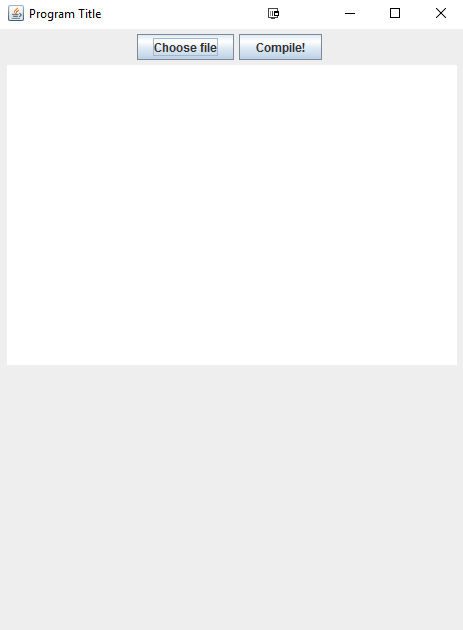
\includegraphics[scale=0.5]{resources/Images/Udklip.PNG}
\caption{The \lang{} GUI.)}\label{fig:GUI}
\end{figure}

The following section describes and presents the tests made on the \lang{} compiler.